\documentclass[11pt]{article}
\usepackage[utf8]{inputenc}
\usepackage[T1]{fontenc}
\usepackage{amsmath}
\usepackage{amssymb}
\usepackage{multicol}
\usepackage{geometry}
\usepackage{tikz}
\usepackage{enumitem}
\usepackage{xcolor}
\usepackage{titlesec}

% Configurações de layout
\geometry{a4paper, left=1cm, right=1cm, top=0.5cm, bottom=1.2cm}
\setlength{\columnseprule}{0.4pt}

% Cores para títulos
\titleformat{\section}{\normalfont\Large\bfseries\color{blue}}{\thesection}{1em}{}
\titleformat{\subsection}{\normalfont\large\bfseries\color{red}}{\thesubsection}{1em}{}

\title{\textcolor{red}{Primeiro Trimestre: Matemática Financeira\\
    Juros Simples - Resoluções Comentadas}}
\author{Professor: Jefferson}
\date{}

\begin{document}

\maketitle
\vspace{-1cm}

\begin{multicols}{2}

\section*{Exercícios Básicos - Juros Simples}

\begin{enumerate}[leftmargin=*]

\item Calcule os juros simples:
\begin{enumerate}[label=\alph*)]
\item $C = R\$ 1000$, $i = 2\%$ a.m., $t = 6$ meses
\textcolor{blue}{Fórmula: $J = C \cdot i \cdot t$\\
Substituindo: $J = 1000 \cdot \frac{2}{100} \cdot 6 = 1000 \cdot 0,02 \cdot 6$\\
$J = 20 \cdot 6 = R\$ 120$}
\item $C = R\$ 500$, $i = 1,5\%$ a.m., $t = 1$ ano
\textcolor{blue}{Atenção: taxa mensal e tempo em anos. Converter 1 ano = 12 meses.\\
$J = 500 \cdot \frac{1,5}{100} \cdot 12 = 500 \cdot 0,015 \cdot 12$\\
$J = 7,5 \cdot 12 = R\$ 90$}
\item $C = R\$ 2000$, $i = 10\%$ a.a., $t = 2$ anos
\textcolor{blue}{Taxa e tempo já estão na mesma unidade (anos).\\
$J = 2000 \cdot \frac{10}{100} \cdot 2 = 2000 \cdot 0,10 \cdot 2$\\
$J = 200 \cdot 2 = R\$ 400$}
\end{enumerate}

\item Calcule o montante a juros simples:
\begin{enumerate}[label=\alph*)]
\item $C = R\$ 800$, $i = 3\%$ a.m., $t = 5$ meses
\textcolor{blue}{Fórmula do montante: $M = C \cdot (1 + i \cdot t)$\\
$M = 800 \cdot (1 + 0,03 \cdot 5) = 800 \cdot (1 + 0,15)$\\
$M = 800 \cdot 1,15 = R\$ 920$}
\item $C = R\$ 1500$, $i = 2\%$ a.m., $t = 8$ meses
\textcolor{blue}{$M = 1500 \cdot (1 + 0,02 \cdot 8) = 1500 \cdot (1 + 0,16)$\\
$M = 1500 \cdot 1,16 = R\$ 1740$}
\item $C = R\$ 3000$, $i = 15\%$ a.a., $t = 3$ anos
\textcolor{blue}{$M = 3000 \cdot (1 + 0,15 \cdot 3) = 3000 \cdot (1 + 0,45)$\\
$M = 3000 \cdot 1,45 = R\$ 4350$}
\end{enumerate}

\item Complete a tabela (juros simples):
\begin{center}
\renewcommand{\arraystretch}{1.2}
\begin{tabular}{|c|c|c|c|}
\hline
\textbf{C} & \textbf{i} & \textbf{t} & \textbf{J} \\
\hline
R\$ 1000 & 2\% a.m. & 6 meses & \textcolor{blue}{R\$ 120} \\
\hline
R\$ 500 & 12\% a.a. & 2 anos & \textcolor{blue}{R\$ 120} \\
\hline
R\$ 2000 & 1,5\% a.m. & 1 ano & \textcolor{blue}{R\$ 360} \\
\hline
\end{tabular}
\end{center}
\item Problemas práticos:
\begin{enumerate}[label=\alph*)]
\item João aplicou R\$ 800 a juros simples de 3\% a.m. por 5 meses. Qual o montante?
\textcolor{blue}{$M = C(1+it) = 800(1+0,03\cdot5) = 800(1+0,15)$\\
$M = 800 \cdot 1,15 = R\$ 920$}
\item Um capital de R\$ 1200 rendeu R\$ 288 em 1 ano. Qual a taxa anual?
\textcolor{blue}{Isolando a taxa: $i = \dfrac{J}{C \cdot t} = \dfrac{288}{1200 \cdot 1}$\\
$i = \dfrac{288}{1200} = 0,24 = 24\%$ a.a.}
\item Qual o tempo necessário para R\$ 2000 render R\$ 600 a 5\% a.m.?
\textcolor{blue}{Isolando o tempo: $t = \dfrac{J}{C \cdot i} = \dfrac{600}{2000 \cdot 0,05}$\\
$t = \dfrac{600}{100} = 6$ meses}
\end{enumerate}
\end{enumerate}

\section*{Exercícios Intermediários}

\begin{enumerate}[leftmargin=*, start=5]

\item Calcule a taxa mensal equivalente a:
\begin{enumerate}[label=\alph*)]
\item 12\% a.a.
\textcolor{blue}{Em juros simples, as taxas são proporcionais. Dividimos por 12:\\
$i_{mensal} = \dfrac{12\%}{12} = 1\%$ a.m.}
\item 24\% a.a.
\textcolor{blue}{$i_{mensal} = \dfrac{24\%}{12} = 2\%$ a.m.}
\item 30\% a.a.
\textcolor{blue}{$i_{mensal} = \dfrac{30\%}{12} = 2,5\%$ a.m.}
\end{enumerate}

\item Um capital de R\$ 2000 foi aplicado a juros simples:
\begin{enumerate}[label=\alph*)]
\item Rendendo R\$ 600 em 1 ano. Qual a taxa anual?
\textcolor{blue}{$i = \dfrac{J}{C \cdot t} = \dfrac{600}{2000 \cdot 1} = 0,30 = 30\%$ a.a.}
\item Rendendo R\$ 450 em 9 meses. Qual a taxa mensal?
\textcolor{blue}{$i = \dfrac{450}{2000 \cdot 9} = \dfrac{450}{18000} = 0,025 = 2,5\%$ a.m.}
\item Qual o montante após 2 anos à taxa de 8\% a.a.?
\textcolor{blue}{$M = 2000 \cdot (1 + 0,08 \cdot 2) = 2000 \cdot (1 + 0,16)$\\
$M = 2000 \cdot 1,16 = R\$ 2320$}
\end{enumerate}

\item Determine o tempo necessário:
\begin{enumerate}[label=\alph*)]
\item Duplicar um capital a 10\% a.a.
\textcolor{blue}{Montante = 2 vezes o capital: $2C = C(1+0,10t)$\\
Dividindo por C: $2 = 1 + 0,10t$\\
$0,10t = 1 \Rightarrow t = 10$ anos}
\item Triplicar um capital a 5\% a.m.
\textcolor{blue}{$3C = C(1+0,05t) \Rightarrow 3 = 1 + 0,05t$\\
$0,05t = 2 \Rightarrow t = 40$ meses}
\item R\$ 1500 render R\$ 600 a 2\% a.m.
\textcolor{blue}{$t = \dfrac{J}{C \cdot i} = \dfrac{600}{1500 \cdot 0,02} = \dfrac{600}{30} = 20$ meses}
\end{enumerate}

\item Problemas contextualizados:
\begin{enumerate}[label=\alph*)]
\item Empréstimo de R\$ 5000 a 2\% a.m. por 10 meses. Qual o total a pagar?
\textcolor{blue}{Total = Montante: $M = 5000(1+0,02\cdot10) = 5000(1+0,20)$\\
$M = 5000 \cdot 1,20 = R\$ 6000$}
\item Uma aplicação de R\$ 3000 rendeu R\$ 450 em 6 meses. Qual a taxa mensal?
\textcolor{blue}{$i = \dfrac{450}{3000 \cdot 6} = \dfrac{450}{18000} = 0,025 = 2,5\%$ a.m.}
\item Quantos meses são necessários para R\$ 2000 virar R\$ 2600 a 1,5\% a.m.?
\textcolor{blue}{$2600 = 2000(1+0,015t) \Rightarrow \dfrac{2600}{2000} = 1+0,015t$\\
$1,3 = 1+0,015t \Rightarrow 0,015t = 0,3 \Rightarrow t = 20$ meses}
\end{enumerate}

\item Análise de gráfico:
\begin{center}
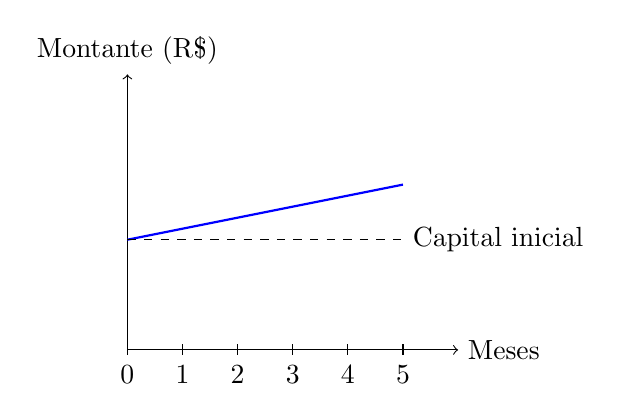
\begin{tikzpicture}[scale=0.7]
\draw[->] (0,0) -- (6,0) node[right] {Meses};
\draw[->] (0,0) -- (0,5) node[above] {Montante (R\$)};
\draw[blue, thick] (0,2) -- (1,2.2) -- (2,2.4) -- (3,2.6) -- (4,2.8) -- (5,3.0);
\foreach \x in {0,1,2,3,4,5} \draw (\x,0.1) -- (\x,-0.1) node[below] {\x};
\draw[dashed] (0,2) -- (5,2) node[right] {Capital inicial};
\end{tikzpicture}
\end{center}
\begin{enumerate}[label=\alph*)]
\item Qual o capital inicial?
\textcolor{blue}{No gráfico, quando $t=0$, o montante é R\$ 2000. Portanto, $C = R\$ 2000$.}
\item Qual a taxa mensal?
\textcolor{blue}{Em 1 mês, o montante foi de R\$2000 para R\$2200.\\ Juros = R\$200.\\
$i = \dfrac{J}{C \cdot t} = \dfrac{200}{2000 \cdot 1} = 0,10 = 10\%$ a.m.}
\item Qual o montante após 8 meses?
\textcolor{blue}{$M = 2000 \cdot (1 + 0,10 \cdot 8) = 2000 \cdot (1 + 0,80)$\\
$M = 2000 \cdot 1,80 = R\$ 3600$}
\end{enumerate}
\end{enumerate}

\section*{Problemas Avançados}

\begin{enumerate}[leftmargin=*, start=9]

\item Regras práticas:
\begin{enumerate}[label=\alph*)]
\item Um capital aplicado a juros simples dobra em 10 anos. Qual a taxa?
\textcolor{blue}{Dobrar: $M=2C$. Então: $2C = C(1+i\cdot10)$\\
$2 = 1 + 10i \Rightarrow 10i = 1 \Rightarrow i = 0,10 = 10\%$ a.a.}
\item Em quanto tempo um capital quadruplica a 5\% a.m.?
\textcolor{blue}{Quadruplicar: $M=4C$. $4C = C(1+0,05t)$\\
$4 = 1 + 0,05t \Rightarrow 0,05t = 3 \Rightarrow t = 60$ meses}
\item Qual capital rende R\$ 1000 em 8 meses a 2,5\% a.m.?
\textcolor{blue}{$C = \dfrac{J}{i \cdot t} = \dfrac{1000}{0,025 \cdot 8} = \dfrac{1000}{0,2} = R\$ 5000$}
\end{enumerate}

\item Comparação de propostas:
\begin{enumerate}[label=\alph*)]
\item Banco A: R\$ 5000, 2,2\% a.m., 12 meses
\item Banco B: R\$ 5000, 2,5\% a.m., 10 meses
\item Qual cobra menos juros?
\textcolor{blue}{$J_A = 5000 \cdot 0,022 \cdot 12 = 5000 \cdot 0,264 = R\$ 1320$\\
$J_B = 5000 \cdot 0,025 \cdot 10 = 5000 \cdot 0,25 = R\$ 1250$\\
Banco B cobra R\$ 70 a menos que o Banco A. Resposta: Banco B.}
\end{enumerate}

\item Problema de lógica:
\begin{enumerate}[label=\alph*)]
\item Um capital aplicado a juros simples duplica em 8 anos. Em quanto tempo triplicaria?
\textcolor{blue}{Primeiro, encontramos a taxa: $2C = C(1+i\cdot8) \Rightarrow 1=8i \Rightarrow i=12,5\%$ a.a.\\
Agora para triplicar: $3C = C(1+0,125t) \Rightarrow 2 = 0,125t$\\
$t = \dfrac{2}{0,125} = 16$ anos}
\item Se R\$ 4000 rende R\$ 1000 em 5 meses, qual a taxa anual?
\textcolor{blue}{Taxa mensal: $i_{mensal} = \dfrac{1000}{4000\cdot5} = \dfrac{1000}{20000}=0,05=5\%$ a.m.\\
Taxa anual: $i_{anual} = 5\% \cdot 12 = 60\%$ a.a.}
\end{enumerate}

\item Desafio final:
\begin{enumerate}[label=\alph*)]
\item Determine o montante para depósitos mensais iguais de R\$ 100 a juros simples de 1\% a.m. após 12 meses.
\textcolor{blue}{1º depósito (mês 1): rende juros por 12 meses: $100(1+0,01\cdot12)$\\
2º depósito (mês 2): rende por 11 meses: $100(1+0,01\cdot11)$\\
...\\
12º depósito (mês 12): rende por 1 mês: $100(1+0,01\cdot1)$\\
Somando: $M = 100[12 + 0,01(12+11+...+1)]$\\
$12+11+...+1 = \dfrac{12\cdot13}{2} = 78$\\
$M = 100[12 + 0,01\cdot78] = 100[12 + 0,78] = 100 \cdot 12,78 = R\$ 1278$}
\item Compare: R\$ 1000 a 2\% a.m. por 2 anos vs R\$ 1000 a 1,8\% a.m. por 2 anos
\textcolor{blue}{2 anos = 24 meses.\\
Opção 1: $M_1 = 1000(1+0,02\cdot24) = 1000(1+0,48) = 1000 \cdot 1,48 = R\$ 1480$\\
Opção 2: $M_2 = 1000(1+0,018\cdot24) = 1000(1+0,432) = 1000 \cdot 1,432 = R\$ 1432$\\
Diferença: $1480 - 1432 = R\$ 48$ a mais na primeira opção.}
\end{enumerate}

\end{enumerate}

\end{multicols}

\end{document}
